\section{U-turn}
%
The second developed example is a simple U-shaped turn. In the specific, the track, is composed by three sections. The first is a straight line of $200\,\si{\metre}$, followed by a left turn of $180\,\si{\degree}$ with radius of curvature equal to $75\,\si{\metre}$. Finally at the exit of the curve there is a straight line equal to the first one ($200\,\si{\metre}$). The road is $12\,\si{\metre}$ wide as usual race circuit.\\
This example is particularly interesting test bench for the model and the optimal control set-up. In fact, a lot of real circuits have in their track an U-shaped turn even if not such regular an symmetric as in the example devised.\\
The problem that the author aim to solve is to travel this simple track at the peak performance of the motorcycle. Therefore starting as fast as the motorcycle can and travel, leaving free initial and final condition.
%
\subsection{Solution approach}
%
This problem cannot be solved in a straight forward fashion. It it complex and not converging without the right guess of state controls and lagrange multipliers.\\
Therefore, the solution is reached using homotopy. At first step the solution is found imposing the well known steady state in the mayer term while the final condition is left free. The second step, as in the other case is to impose initial and final condition equal. After the initial conditions are slowly freed. At the last step the tolerances of the penalties are pushed to reach the maximum performance.
%
\subsection{Results and comparison}
%
Similarly to the case of straight running, the torque control is able to reach more aggressive manoeuvre. As highlighted in figure \ref{fig:U1a} the torque control can reach higher starting velocity, then a equal minimum velocity in cornering is reached. At the exit of the curve the torque control reach again an higher velocity. The higher performance of the torque control can be seen in figure \ref{fig:U1b} in the lateral velocity but it is more unstable and oscillatory.\\
%
\begin{figure}[t]
    \begin{subfigure}{0.5\linewidth}
        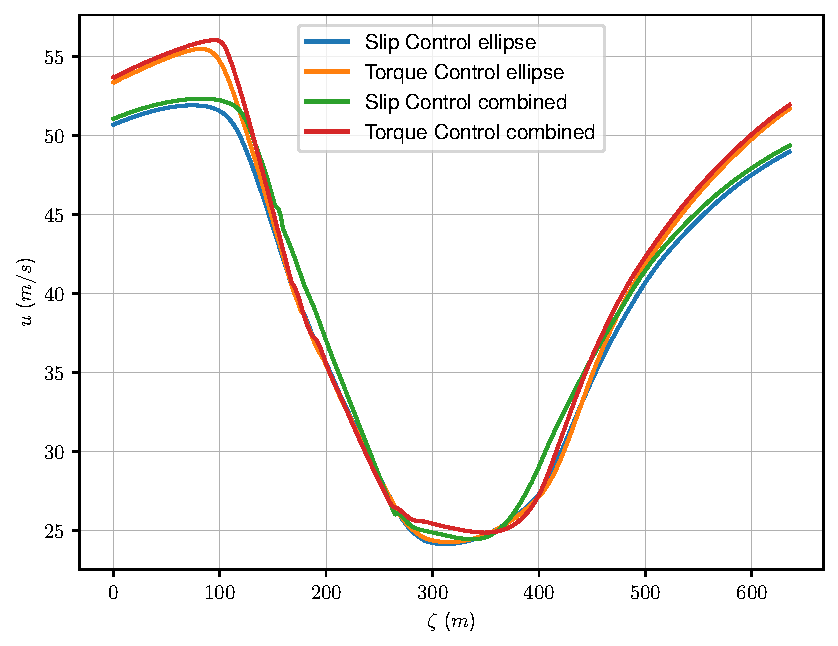
\includegraphics[width=\linewidth]{U-turn/u_U_confront.pdf}
        \caption{Longitudinal velocity}
        \label{fig:U1a}
    \end{subfigure}%
    \begin{subfigure}{0.5\linewidth}
        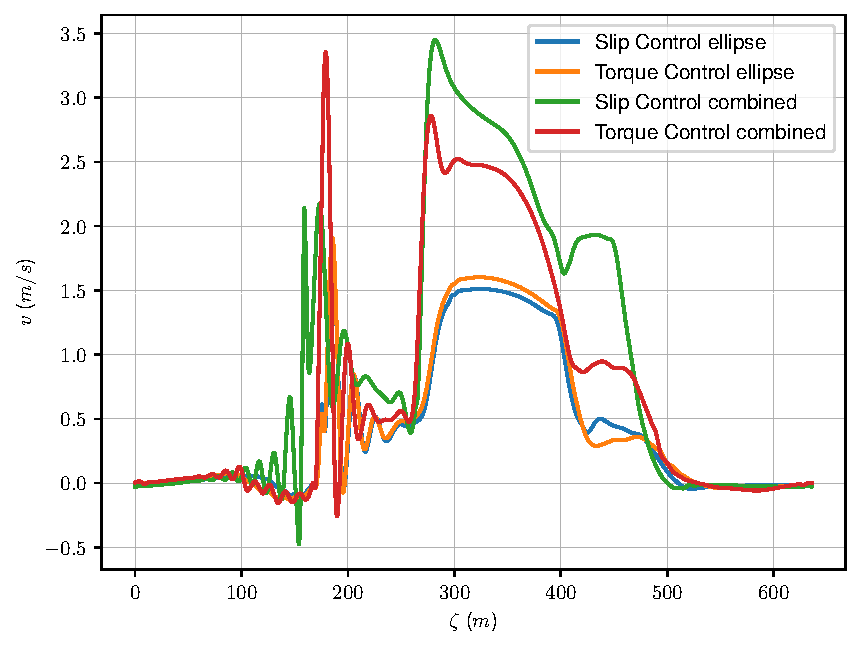
\includegraphics[width=\linewidth]{U-turn/v_U_confront.pdf}
        \caption{Lateral velocity}
        \label{fig:U1b}
    \end{subfigure}
    \caption{Confront of velocity in U-turn}
\end{figure}
%
%
\begin{figure}[t]
    \begin{subfigure}{0.5\linewidth}
        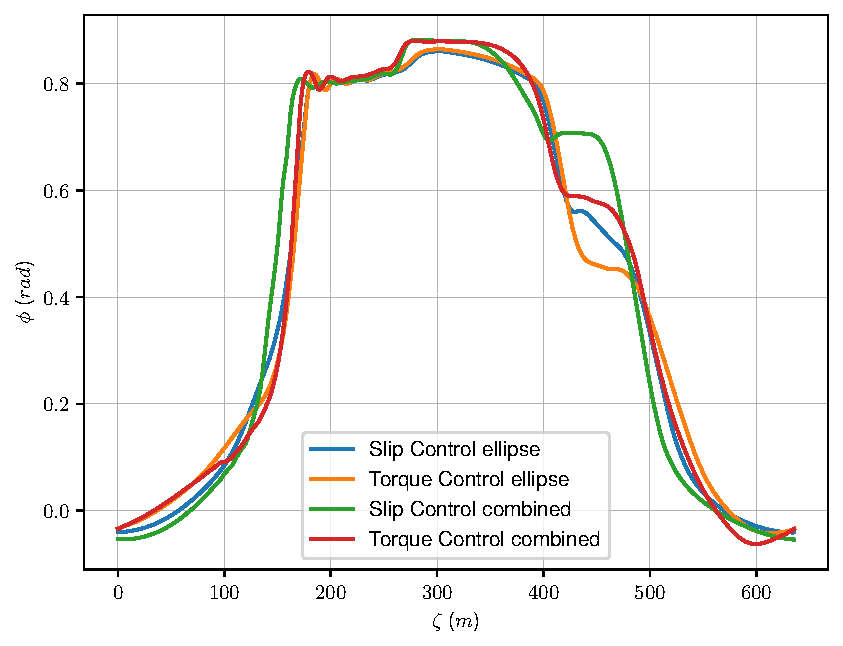
\includegraphics[width=\linewidth]{U-turn/phi_U_confront.pdf}
        \caption{Roll angle}
        \label{fig:U2a}
    \end{subfigure}%
    \begin{subfigure}{0.5\linewidth}
        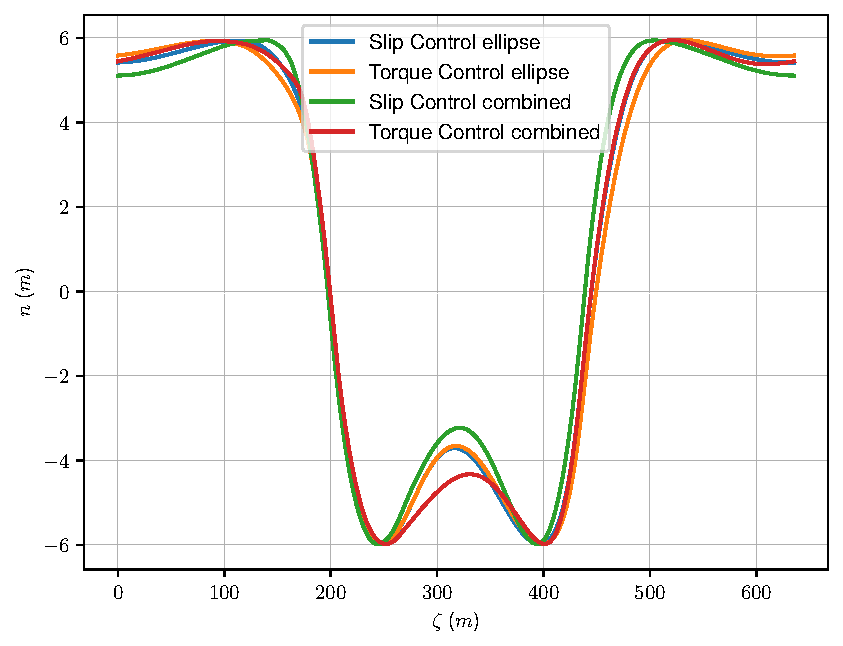
\includegraphics[width=\linewidth]{U-turn/n_U_confront.pdf}
        \caption{centreline deviation}
        \label{fig:U2b}
    \end{subfigure}
    \caption{Confront of roll angle and centreline deviation in U-turn}
\end{figure}
%
The trajectory followed in the four cases is almost the same. In fact in in figure \ref{fig:U2b} the deviations from the centre line are really close to each other.\\
Moreover, the trajectory calculated is consistent with real driver manoeuvres. The driver will  start at the right border, lean into the corner and touch two tangent points in the inside border of the turn. Then again reach the external border in acceleration.(figure \ref{fig:UTrajectory})\\
Another important key performance index is the roll angle and it shows a similar behaviour in all four models (figure \ref{fig:U2a}). The roll angle difference is only at the exit of the turn and it can be seen both in figure \ref{fig:U2a} and \ref{fig:U2b}.\\
%
\begin{figure}[!ht]
    \centering
    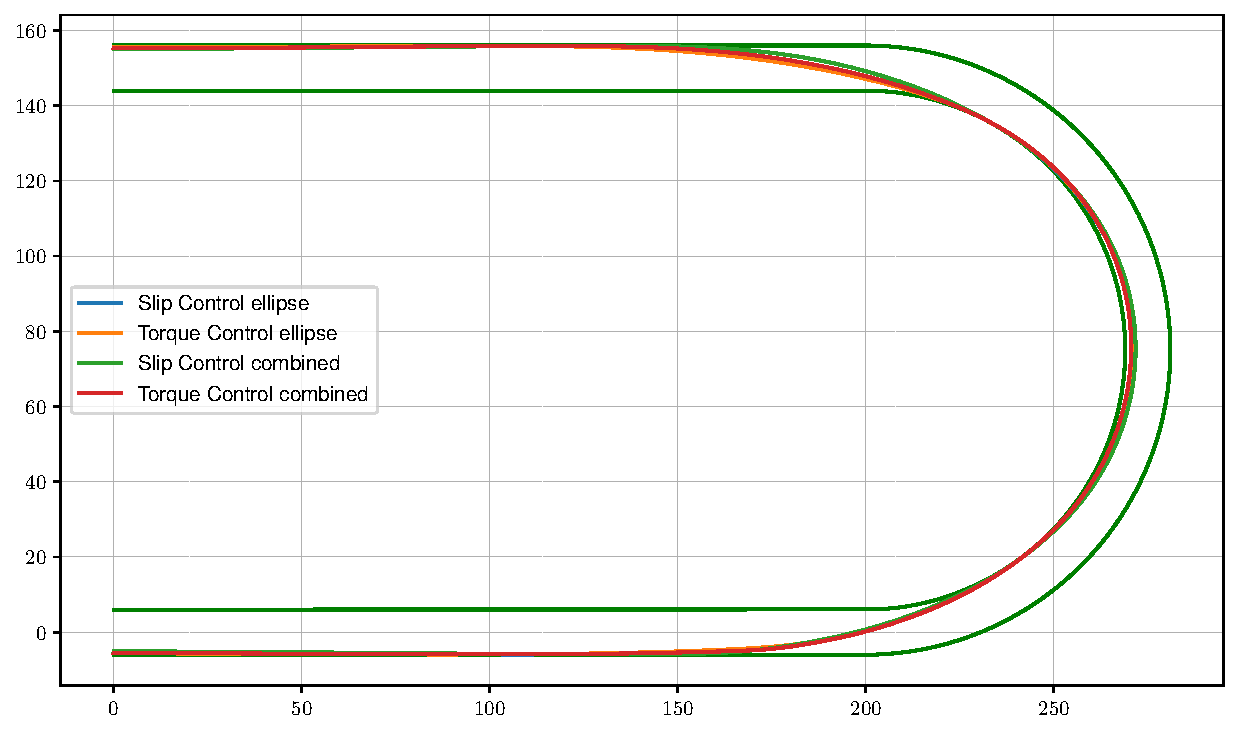
\includegraphics[width=\linewidth]{U-turn/Track_U_confront.pdf}
    \caption{Trajectory in U-turn}
    \label{fig:UTrajectory}
\end{figure}
%
In vehicles dynamics it is important to confront the ellipse derived from the longitudinal and lateral forces normalised with the vertical load for both rear and front wheels. In particular in this case we can clearly see that in figure \ref{fig:UEa} and \ref{fig:UEb} even if it is not such significant in only one turn.\\
%
\begin{figure}[!ht]
    \begin{subfigure}{0.5\linewidth}
        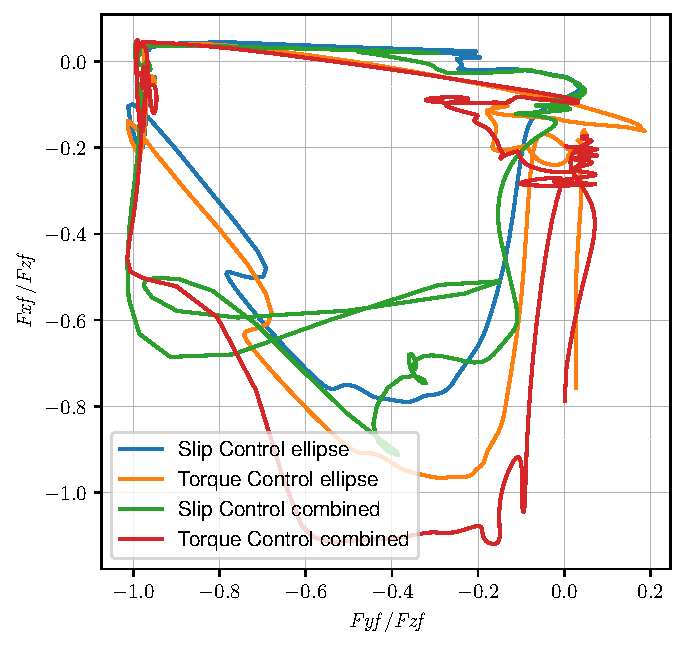
\includegraphics[width=\linewidth]{U-turn/EFront_U_confront.pdf}
        \caption{Front}
        \label{fig:UEa}
    \end{subfigure}%
    \begin{subfigure}{0.5\linewidth}
        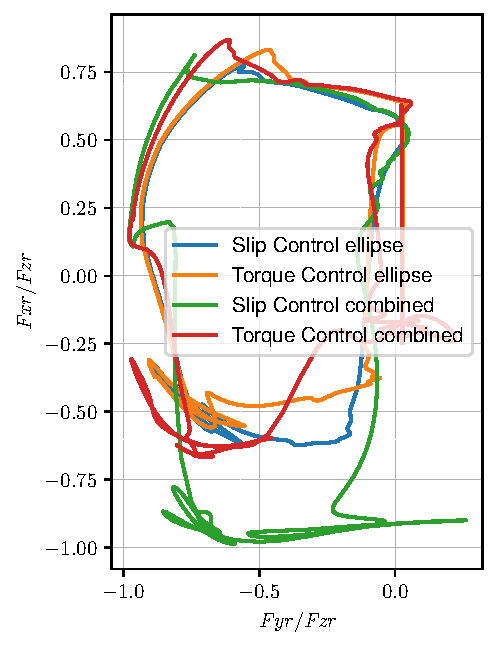
\includegraphics[width=\linewidth]{U-turn/ERear_U_confront.pdf}
        \caption{Rear}
        \label{fig:UEb}
    \end{subfigure}
    \caption{Ellipse of adherence U-turn}
\end{figure}
%